\chapter{Concepts and Architecture}
\label{chap:concepts_and_architecture}

In this chapter we discuss the relevant concepts used throughout this thesis and describe how they fit together into the high level system architecture of our
application. First, it describes how our application makes use of a multimedia retrieval systems in order to manage a multimedia database and to be able to search such a database for certain 3D models.
Then, it explains two representations of 3D models and why they are relevant to this thesis. Lastly, it describes how our application makes use of virtual reality and how our novel virtual reality 3D model retrieval system combines all these topics.

\section{Multimedia Retrieval}
\label{sec:multimedia_retrieval_concept}

Multimedia retrieval has become an ever more important topic over the last decades. As the name implies, multimedia retrieval entails the retrieval of various different media such as text, images, video and audio but also
3D models. The goal is to allow the user to find such media based on an example input or a subset of the desired result, i.e. retrieve them from some multimedia database.\\
The DBIS research group\footnote{\url{https://dbis.dmi.unibas.ch/}} is working on such a system called Cineast. Cineast provides the backend functionality for multimedia retrieval queries and Vitrivr NG provides a web
based frontend to enable users to build queries. Currently it supports queries for text, images, video, audio and 3D models.\\
In order to run multimedia queries a multimedia database is required to store the data to compare media. Cineast currently supports the Cottontail DB column store database for multimedia retrieval which also being developed by the DBIS research group.\\
The focus of this thesis is on 3D model retrieval which is also part of multimedia retrieval. Research in this area has so far focused on building 3D model queries from example images, sketches or common 3D model file formats.
In order to create one of these 3D model files the user requires a seperate sculpting program and needs to learn how to use it.\\
Multimedia retrieval systems commonly rely on the Vector Space Model [\todoMissing{Missing ref; \url{https://dl.acm.org/doi/10.1145/361219.361220}}] in order to compare media for similarity. To goal is to find an algorithm to convert the media into a high dimensional feature vector $D_i = (d_{i1}, d_{i2}, ..., d_{in})$, such that the feature vectors of similar media are as close to each other as possible and those of dissimilar media respectively as far away from each other as possible. How close two feature vectors are to each other is determined by a distance function $s(D_i, D_j)$. Retrieving a list of media similar to some input is then a matter of using a $k$-nearest neighbors search [\todoMissing{Missing ref; \url{https://www.cadmo.ethz.ch/education/lectures/FS18/SDBS/papers/IndykM-curse.pdf}}] algorithm to find the $k$ closest feature vectors to the input media's feature vector.\\
For example to compare a 3D model for similarity one may use an algorithm that converts the 3D model into an n-dimensional real-valued feature vector $D_i$, such that the feature vectors of 3D models with a similar geometry or shape are close to each other. Then use $s(D_i, D_j) = \lVert D_i - D_j \rVert$, which corresponds to the L2 distance between $D_i$ and $D_j$, to obtain a metric for the similarity of two feature vectors, respectively their 3D models.

\section{REST API}
\label{sec:rest_api_concept}

In order for a multimedia retrieval system to become useful it needs to provide some interface through which other applications can access its functionality. This is what's commonly known as an application programming interface (API). One such type of APIs are REST APIs, an acronym for Representational State Transfer. These REST APIs aim to communicate between two programs via requests and responses over the HTTP web protocol. The following incomplete list should give an insight into how REST APIs operate - according to R. Fielding [\todoMissing{Missing ref; \url{https://www.ics.uci.edu/~fielding/pubs/dissertation/rest_arch_style.htm}}] REST APIs follow these and some more principles:
\begin{itemize}
	\item Client-Server: User interface concerns should be separated from data storage concerns.
	\item Stateless: Communication must be stateless. All information required for a request to be understood must be included in said request.
	\item Cache: Responses' data must be labeled whether the data can be cached on the client side or not. If it is chacheable the client may reuse the same data for future equivalent requests.
	\item Uniform Interface: The REST API should form a uniform interface. Said interface should remain the same independent of the back-end implementation.
	\item And several other principles.
\end{itemize}
Usually REST requests are exclusively executed by sending an HTTP \textit{GET}, \textit{PUT}, \textit{POST} or \textit{DELETE} request through certain server provided URLs.\\

\section{3D Models}
\label{sec:3D_models}

Usually virtual 3D model consist of one or multiple polygon meshes. Formally, a polygon mesh consist of a list of vertices $\mathcal{V} = \{\mathcal{P}, ...\}$. Each vertex has at least a position $\mathcal{P} = (x, y, z)$, but can also contain other attributes such as a color. This list of vertices is then used to define the surface of the mesh. The polygons of choice to represent the mesh's surface are usually triangles, where each triplet of consecutive vertices of the mesh forms one triangle. Triangles are the primary choice for representing 3D model surfaces in computer graphics because they have some desirable properties like always being planar. In addition to that modern hardware is built mostly around rendering triangles and is thus very fast at it.\\
However, such 3D models that consist of polygon meshes are restricted to representing surfaces. They cannot represent a volume, since there is no way to specify what's inside a mesh. Another way to represent 3D models, but in a volumetric way, is discussed in Section \ref{sec:voxels_concept}.

\section{Voxels}
\label{sec:voxels_concept}
%What are voxels, purpose, hermite data, etc.

Our application provides a 3D sculpting module and thus needs a suitable virtual representation of the sculptures. Usually 3D model formats only store the surface of a sculpture, but our application requires the sculptures to be
truly volumetric and not just an empty shell, so that when the user removes some material from the sculpture they should be able to see the material filling the inside of the sculpture.\\
The foundation of the sculpting module is thus based on voxels. In the most basic sense a voxel represents a value on a regular grid in 3D space [\todoMissing{Missing ref; Wikipedia}].
The value contained in a voxel usually describes which material it is made of, but can also contain additional data, e.g. to describe the shape of the voxel.\\
These voxels are very useful to represent volumetric structures, such as sculptures or terrain, since they fill the 3D space and each voxel represents one volume element. One can imagine voxels being like LEGO bricks with which
the sculptures are built, or the analog to atoms on a much larger scale.\\
Compared to polygon mesh based 3D models these voxels have the advantage of being able to define the inside of a 3D model. This however comes at a cost of higher memory usage, since not only the surface must be defined but also what's inside. Futhermore, current GPU hardware is lacking extensive hardware support for voxels and thus they are not the primary choice to represent 3D models. In the recent years however voxels have gained a lot of popularity in other areas of computer graphics, especially for lighting calculations such as global illumination [\todoMissing{Missing ref; https://dl.acm.org/doi/pdf/10.1145/1944745.1944763}] or ambient occlusion [\todoMissing{Missing ref; https://developer.nvidia.com/vxao-voxel-ambient-occlusion}].

\subsection{Voxelization}

\hfill

\begin{figure}
\centering
\captionsetup{width=0.8\textwidth}
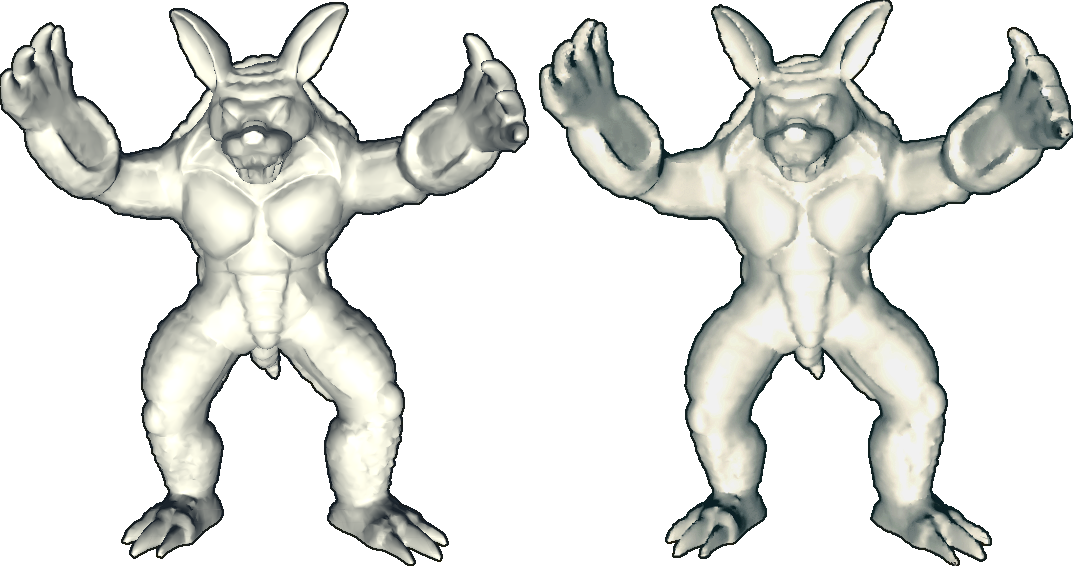
\includegraphics[width=0.75\textwidth]{voxelizer_example_transparent_3.png}
\caption{The Stanford Armadillo mesh\protect\footnotemark  (left) and its voxel representation at a resolution of 128x128x128 voxels (right).}
\label{fig:voxelizer_example}
\end{figure}
\footnotetext{\url{http://graphics.stanford.edu/data/3Dscanrep/}}

An important part of multimedial retrieval is the ability to take query results and reuse them to formulate a new, refined, query. In the context of this thesis multimedia retrieval
is only concerned with polygonal meshes. To facilitate the modification of such polygonal meshes our application includes a voxelizer module. The voxelizer takes a polygonal
mesh as input and converts it into a suitable voxel representation to enable the user to edit the model volumetrically. Since
our voxels contain not only the voxel material, but also the surface normals, we can reconstruct the mesh from our voxels while keeping most of the mesh's features intact with high accuracy, given
a large enough voxel grid with sufficient resolution. In practice a resolution of 128x128x128 seems to be sufficient for most models that aren't highly detailed or noisy.
Fig. \ref{fig:voxelizer_example} depicts an example of a mesh that has been converted to a voxel grid using an algorithm described in Section \ref{sec:voxelizer}.

\subsection{Isosurface Polygonization}

Since the voxels are just an internal volumetric representation an algorithm is required to convert them into a representation that a computer can display on the monitor. Usually the representation of choice are meshes, as described in \ref{sec:3D_models}, since that's what modern GPU's are specialized in. In general these kinds of algorithms are called isosurface polygonization algorithms, since originally they were conceived to convert implicit functions, or e.g.
computed tomography (CT) density fields, into a polygonal surface. The prefix "iso-" means equal, hence the word "isosurface" comes from the fact that the implicit function value or density is the same everywhere on the polygonal surface. There are some variants that do not directly work off of density fields but instead some intermediary representation like Hermite data which will be discussed in detail later on.

\begin{figure}
\centering
\captionsetup{width=0.8\textwidth}
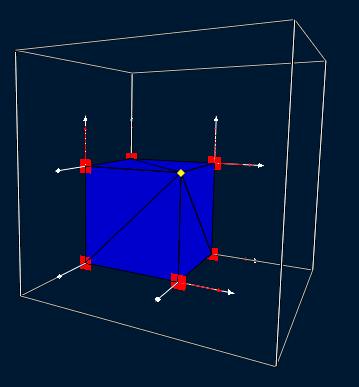
\includegraphics[width=0.35\textwidth]{voxel_scene_cube.png}
\caption{A polygonized voxel cell (white) containing the polygon surface of a cube's corner (blue) with a sharp feature (yellow).}
\label{fig:polygonized_cube_voxel_cell}
\end{figure}

%Method for converting voxels into meshes, some common algorithms as examples

The two main groups of isosurface polygonization alrogithms are the primal (\todoMissing{Missing ref; MC etc.}) and dual (\todoMissing{Missing ref; DC, CMS, etc.}) contouring algorithms.
Most of these algorithms cannot polygonize a single voxel by itself, but instead require a cell consisting of eight voxels, usually arranged in the form
of a cube. Primal and dual contouring algorithms differ in that the primal variants place polygon vertices somewhere on the cell's edges and the dual variants
place them not on the edges but somewhere within the cell's volume. Therefore dual contouring algorithms have the advantage that they can more reliably polygonize
surfaces with sharp features, such as e.g. the corners of a cube. Primal contouring algorithms can also polygonize sharp features in certain cases, however only
if said sharp feature lies exactly on a cell's edge. Fig. \ref{fig:polygonized_cube_voxel_cell} depicts a polygonized voxel cell where the sharp feature lies within
the voxel cell.\\
Marching Cubes [\todoMissing{Missing ref}] (MC), a primal contouring algorithm, checks whether the material at each corner of the voxel cell is filled or empty and then 
packs all 8 resulting booleans into a single 8 bit integer. That integer is then used to index into a lookup table that contains which cell edges are to be connected to
each other to form polygons. Vertex positions can either lie on the middle of their respective cell edge or if the voxel contains a density value the vertex position
can be smoothly linearly interpolated.\\
Dual Contouring [\todoMissing{Missing ref}] (DC) uses another approach. A valid voxel cell always contains either no edge with a material, or at least three edges with a material change. If a voxel cell
does contain edges with a material change then Dual Contouring finds the sharp feature that minimizes the squared distance between the sharp feature and all planes spanned
by the normals at the edges with the material changes. In a second pass the generated vertices are then connected between neighboring voxel cells to form polygons.\\
Cubical Marching Squares [\todoMissing{CMS}] (CMS) makes use of both primal and dual contouring features. Much like MC it places vertices on voxel cell edges. However it can also place vertices
on voxel cell faces and within the voxel cell volume, like dual contouring algorithms do. This gives it the advantage that each cell can be polygonized individually while still being able to
reliably polygonize surfaces with sharp features. This algorithm is described in more detail in Section \ref{sec:cms}.

\section{CSG}

\begin{figure}
\centering
\captionsetup{width=0.8\textwidth}
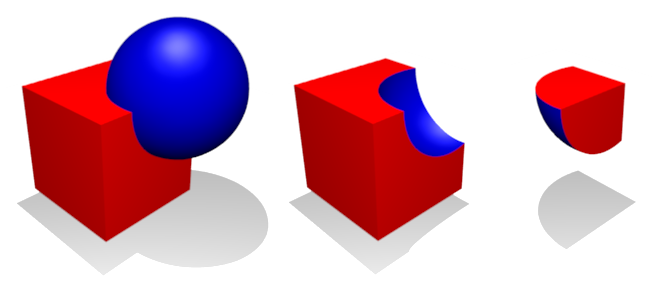
\includegraphics[width=0.6\textwidth]{csg_operations.png}
\caption{Boolean union (left), difference (middle) and intersection (right) of a cube and sphere primitive. Adapted from Wikipedia\protect\footnotemark.}
\label{fig:csg_operations}
\end{figure}
\footnotetext{\url{https://en.wikipedia.org/wiki/Constructive_solid_geometry}}

Constructive Solid Geometry (CSG) is a method to create geometric shapes by constructing them from primitives and a few operations.
The three most common operations are the boolean union ($\cup$), difference ($-$) and intersection ($\cap$) operations are illustrated in Fig. \ref{fig:csg_operations}. With just
those three simple tools and a couple of primitives, e.g. spheres, cubes, cylinders, etc., the user can easily create arbitrary shapes or sculptures.
Additionally CSG need not be restricted to only boolean operations, but can also make use of smooth operations that blend two shapes together in a continuous
manner. In the context of signed distance functions, which will be discussed in Section \ref{sec:signed_distance_functions}, these smooth operations correspond to the smooth minimum and maximum operations.\\
The application developed for this thesis makes extensive use of CSG to enable the users to edit and shape their voxel based sculptures. The union ("add") and
difference ("remove") operations are intuitive and easy to use. Additionally it also provides a "replace" operation that allows the user to replace solid materials inside
a primitive with another material. Logically it is equivalent to $(A-B) \cup (B \cap A)$ where A is the existing sculpture and B is the primitive or bounds within
which solid materials should be replaced with B's material.

\subsection{Signed Distance Functions}
\label{sec:signed_distance_functions}

\begin{figure}
\centering
\captionsetup{width=0.8\textwidth}
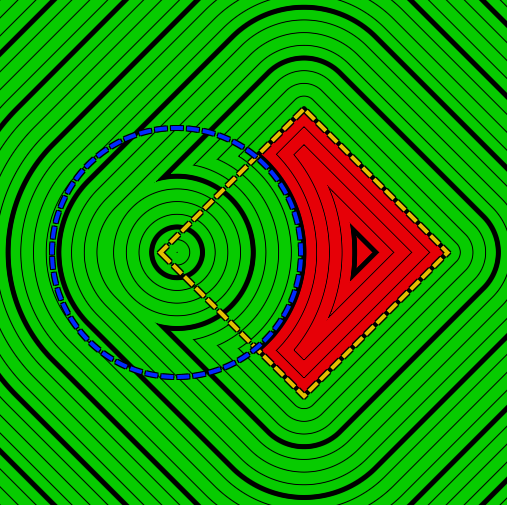
\includegraphics[width=0.4\textwidth]{sdf_difference.png}
\caption{The resulting SDF from subtracting a circle SDF (blue) from a square SDF (yellow). The background is green where the resulting SDF is positive and red otherwise. The black lines represent the isolines of the resulting SDF, i.e. the value is the same everywhere on one of those lines. The subtraction operation results in an inexact SDF as illustrated by the isolines on the left half that are evidently not equidistant from the red area. Adapted from \url{https://sudonull.com/post/1035-Combining-Signed-Distance-Fields-in-2D}}
\label{fig:sdf_difference}
\end{figure}

Signed distance functions (SDF) are mathematical formulas that describe the signed distance between a point and the surface of a certain shape. For points inside the shape the
signed distance is negative. For example it is trivial to derive the signed distance function $f(x,y,z) = \sqrt{x^2 + y^2 + z^2} - r$ of a sphere at $(0, 0, 0)$ from the implicit formula of the sphere's surface, $x^2 + y^2 + z^2 - r^2 = 0$. There exist readily available formulas for SDFs of various shapes, e.g. Inigo Quilez' collection of such functions\footnote{\url{https://iquilezles.org/www/articles/distfunctions/distfunctions.htm}}.\\
SDFs are well suited as a representation of CSG primitives because one can approximate their union and difference by taking the minumum, respectively maximum, of two SDFs. This approach generally works
well and can produce the exact union or difference, however in certain cases it can result in an incorrect approximation, especially for the difference and intersection operations like illustrated in Fig. \ref{fig:sdf_difference}.
For the purposes of this application the SDFs need not be exact, hence we have decided to use SDFs as the representation of our CSG primitives. Additionally since the domain and range are the same for all SDFs, namely
$f\colon \mathbb{R}^3 \mapsto \mathbb{R}$, they can all be treated exactly the same besides their formulas and can be encapsulated as a simple method in code.

%\section{Unity}
%What, why

\section{Virtual Reality}
%What is VR, use cases

Virtual reality (VR) applications and hardware aim to immerse the user into a virtual scene or application as much as possible. This is achieved by the use of a headset with an integrated display that the user wears, whereby all the user can see is the content shown on the integrated display. Furthermore, these headsets track the user's head position and rotation so that it can be precisely reflected in the virtual scene. Another large portion of the immersion also comes from the fact that the integrated display is stereoscopic, i.e. it can trick the user's eyes into seeing the depth of the virtual scene by showing a seperate and slightly offset image of the scene to each eye. In addition to the headset there are also VR controllers that are, similarly to the headset, tracked in 3D space and reflected in the virtual scene. The user can hold these and then precisely control the position of their virtual hands and even use them to manipulate objects in the virtual scene.\\
%Similarly to the "Rubber hand illusion" first described by Botvinick and Cohen [\todoMissing{Missing ref}]
Current 3D sculpting applications usually have a steep learning curve. This comes from the fact that keyboards and computer mice, which serve as the primary human to machine interface, are not intuitive for
sculpting. Modifying parts of a physical clay sculpture by hand is much more intuitive for a human than doing it virtually with a keyboard and mouse, because there is no direct mapping between these actions
and the movement of a mouse or the buttons of a keyboard. There are companies that produce hardware specifically made to alleviate some of these issues, e.g. 3Dconnexion\footnote{\url{https://www.3dconnexion.de/}}, but the issue
of not having a direct mapping mostly persists.\\
This is where virtual reality excels and why it is a crucial part of our application. The VR controllers create a direct mapping between the position and movement of the hands and the ingame sculpting brush. In addition to that
the VR headset also provides a true sense of depth with its stereoscopic display and makes it easier to view the virtual sculpture from all sides because head movement is tracked accurately. When combined these advantages provide
a more immersive experience and hopefully also a more intuitive human machine interface.

\section{System Architecture}
%How all components are connected to each other (cineast, feature module, cottontail, rest api, polygonizer, voxel storage, vr interaction controller, etc.)

\begin{figure}
\centering
\captionsetup{width=0.8\textwidth}
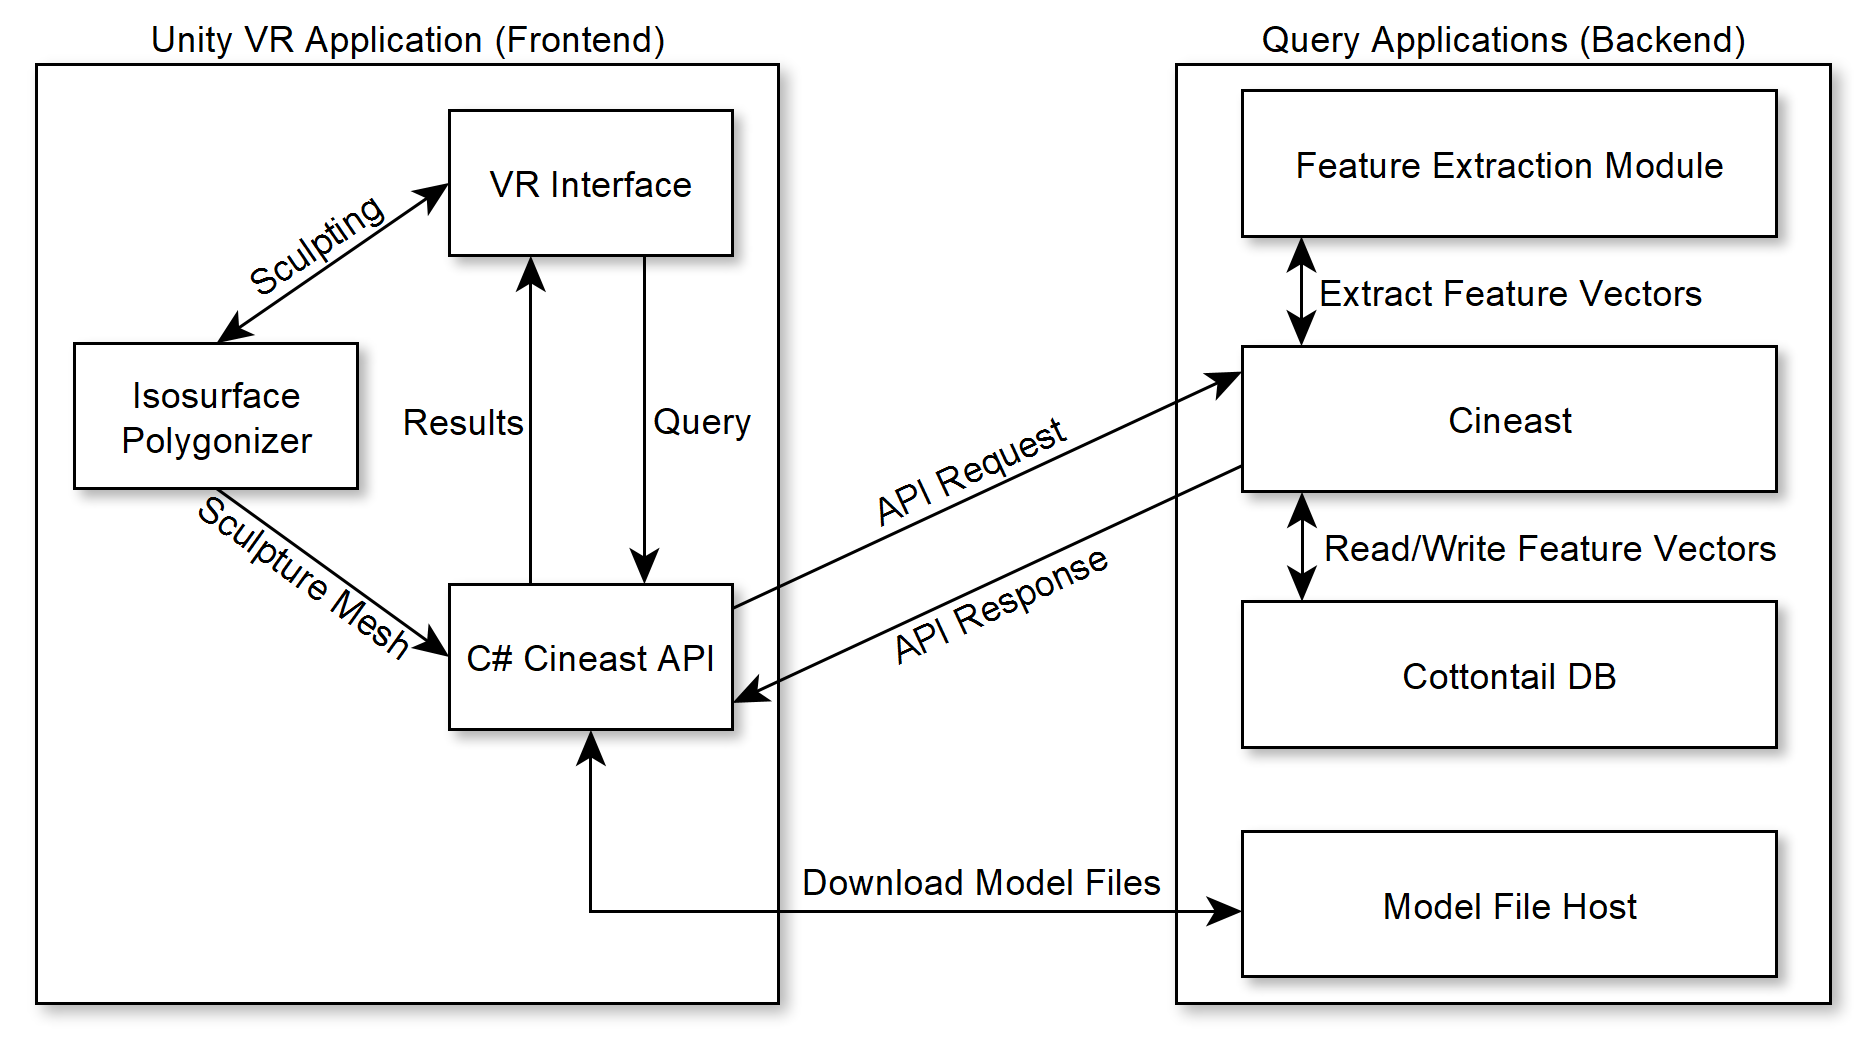
\includegraphics[width=0.8\textwidth]{architecture.png}
\caption{The high level architecture of our system.}
\label{fig:architecture}
\end{figure}

To tie this all together Fig. \ref{fig:architecture} illustrates the high level architecture of our system. The frontend, i.e. our VR application running in the Unity
engine, contains three main components relevant for the querying functionality: the VR interface, isosurface polygonizer and generated C\# Cineast API module.\\
Through the VR interface the user can sculpt using voxels and CSG operations and start queries or view query results. On starting a query from the VR interface the entire sculpture is converted into a single mesh which is then sent to Cineast as a REST API request via the C\# Cineast API.\\
Cineast then tasks the feature extraction module to convert the mesh into a feature vector. This feature vector is then sent over to the Cottontail DB multimedia database to be
compared with the feature vectors of other models. All models in that multimedia database that have a similar feature vector are then scored, ranked and their IDs are sent back to be received by the C\# Cineast API. The C\# Cineast API then uses the received IDs to download the respective model files and hands them over to the VR interface to be displayed.

